\documentclass[3p, authoryear, review]{elsarticle} %review=doublespace preprint=single 5p=2 column
%%% Begin My package additions %%%%%%%%%%%%%%%%%%%
\usepackage[hyphens]{url}

  \journal{Submitted to NARSC 2021} % Sets Journal name


\usepackage{lineno} % add
\providecommand{\tightlist}{%
  \setlength{\itemsep}{0pt}\setlength{\parskip}{0pt}}

\usepackage{graphicx}
\usepackage{booktabs} % book-quality tables
%%%%%%%%%%%%%%%% end my additions to header

\usepackage[T1]{fontenc}
\usepackage{lmodern}
\usepackage{amssymb,amsmath}
\usepackage{ifxetex,ifluatex}
\usepackage{fixltx2e} % provides \textsubscript
% use upquote if available, for straight quotes in verbatim environments
\IfFileExists{upquote.sty}{\usepackage{upquote}}{}
\ifnum 0\ifxetex 1\fi\ifluatex 1\fi=0 % if pdftex
  \usepackage[utf8]{inputenc}
\else % if luatex or xelatex
  \usepackage{fontspec}
  \ifxetex
    \usepackage{xltxtra,xunicode}
  \fi
  \defaultfontfeatures{Mapping=tex-text,Scale=MatchLowercase}
  \newcommand{\euro}{€}
\fi
% use microtype if available
\IfFileExists{microtype.sty}{\usepackage{microtype}}{}
\bibliographystyle{elsarticle-harv}
\usepackage{longtable}
\usepackage{graphicx}
\ifxetex
  \usepackage[setpagesize=false, % page size defined by xetex
              unicode=false, % unicode breaks when used with xetex
              xetex]{hyperref}
\else
  \usepackage[unicode=true]{hyperref}
\fi
\hypersetup{breaklinks=true,
            bookmarks=true,
            pdfauthor={},
            pdftitle={Utility-Based Accessibility to Community Resources: An Application of Location-Based Services Data},
            colorlinks=false,
            urlcolor=blue,
            linkcolor=magenta,
            pdfborder={0 0 0}}
\urlstyle{same}  % don't use monospace font for urls

\setcounter{secnumdepth}{5}
% Pandoc toggle for numbering sections (defaults to be off)

% Pandoc citation processing
\newlength{\cslhangindent}
\setlength{\cslhangindent}{1.5em}
\newlength{\csllabelwidth}
\setlength{\csllabelwidth}{3em}
% for Pandoc 2.8 to 2.10.1
\newenvironment{cslreferences}%
  {}%
  {\par}
% For Pandoc 2.11+
\newenvironment{CSLReferences}[2] % #1 hanging-ident, #2 entry spacing
 {% don't indent paragraphs
  \setlength{\parindent}{0pt}
  % turn on hanging indent if param 1 is 1
  \ifodd #1 \everypar{\setlength{\hangindent}{\cslhangindent}}\ignorespaces\fi
  % set entry spacing
  \ifnum #2 > 0
  \setlength{\parskip}{#2\baselineskip}
  \fi
 }%
 {}
\usepackage{calc}
\newcommand{\CSLBlock}[1]{#1\hfill\break}
\newcommand{\CSLLeftMargin}[1]{\parbox[t]{\csllabelwidth}{#1}}
\newcommand{\CSLRightInline}[1]{\parbox[t]{\linewidth - \csllabelwidth}{#1}\break}
\newcommand{\CSLIndent}[1]{\hspace{\cslhangindent}#1}

% Pandoc header
\usepackage{booktabs}
\usepackage{booktabs}
\usepackage{longtable}
\usepackage{array}
\usepackage{multirow}
\usepackage{wrapfig}
\usepackage{float}
\usepackage{colortbl}
\usepackage{pdflscape}
\usepackage{tabu}
\usepackage{threeparttable}
\usepackage{threeparttablex}
\usepackage[normalem]{ulem}
\usepackage{makecell}
\usepackage{xcolor}



\begin{document}
\begin{frontmatter}

  \title{Utility-Based Accessibility to Community Resources: An Application of Location-Based Services Data}
    \author[BYU]{Gregory Macfarlane\corref{1}}
   \ead{gregmacfarlane@byu.edu} 
    \author[BYU]{Emma Stucki}
   \ead{stuckiemma@gmail.com} 
    \author[BYU]{Michael Copley}
  
    \author[]{}
  
        \cortext[1]{Corresponding Author}
  
  \begin{abstract}
  Understanding who in a community has access to its resources -- parks, libraries,
  grocery stores, etc. -- has profound equity implications, but typical methods
  to understand access to these resources are limited. Travel time buffers require
  researchers to assert mode of access as well as an arbitrary distance threshold;
  further, these methods do not distinguish between destination quality attributes
  in an effective way. In this research, we present a methodology to develop
  utility-based accessibility measures for parks, libraries, and grocery stores
  in Utah County, Utah. The method relies on passive location-based services data
  to model destination choice to these community resources; the destination choice
  model utility functions in turn allow us to develop a picture of regional access
  that is sensitive to: the quality and size of the destination resource;
  continuous (non-binary) travel impedance by multiple modes; and the
  sociodemographic attributes of the traveler. We then use this measure
  to explore equity in access to the specified community resources across
  income level in Utah County.
  \end{abstract}
   \begin{keyword} Accessibility; Passive Data; Location Choice\end{keyword}
 \end{frontmatter}

\hypertarget{intro}{%
\section{Introduction}\label{intro}}

Communities provide important resources to the people who live in them. These
resources might include physical and economic resources
--- shared open space, libraries, commercial establishments, etc. --- as well as less identifiable resources
including a sense of membership and other forms of social capital
(\protect\hyperlink{ref-lochner1999}{Lochner, 1999}). Indeed, access to these resources is a primary reason why
communities exist (\protect\hyperlink{ref-muth1971}{Muth, 1971}), as well as a long-motivating objective in
transportation infrastructure planning (\protect\hyperlink{ref-hansen1959}{Hansen, 1959}).

Given the importance of these community resources, it is not surprising that
so much scholarly attention has been paid to examining the spatial and
socioeconomic variation in access to them (\protect\hyperlink{ref-handy1997}{Handy and Niemeier, 1997}; \protect\hyperlink{ref-witten2003}{Witten et al., 2003}). What
is surprising is the simplistic and arbitrary definition of many
quantitative resource accessibility measures, in spite of the widespread
availability of geographical information systems (GIS) software (\protect\hyperlink{ref-logan2019}{Logan et al., 2019}) and
an understanding that proximity to a resource is not the only consideration
in its use (\protect\hyperlink{ref-dong2006}{Dong et al., 2006}). Individuals do not always shop at the nearest grocery
store, nor do they necessarily perceive an 11-minute walk to a park as
meaningfully different from a 9-minute walk. A measure of access that can
incorporate travel impedance by multiple transportation modes alongside
qualitative attributes of the resources in question would provide a better
theoretical comparison to what people experience and observe in their own
communities. This measure in turn may result in a different understanding
of which groups have or do not have good access --- and therefore in different
policy interventions to resolve the access gap --- than more traditionally used
measures (\protect\hyperlink{ref-logan2019}{Logan et al., 2019}; \protect\hyperlink{ref-macfarlane2020}{Macfarlane et al., 2020}).

In this paper, we develop utility-based access measures to parks, grocery stores, and
libraries in Utah County, Utah. These measures are based in econometric choice
theory relating continuous multimodal travel impedance to attributes of the
resource. The utility preferences are estimated on location-based services data
obtained from a third-party commercial data aggregator. We then use the model
estimates to construct a composite accessibility measure and examine potential
discrepancies between this measure and a more common travel-time buffer
measurement.

The paper begins with a discussion of previous findings relating access to
community resources with social, health, and equity benefits. We then describe
the methodology employed in this research, which makes use of novel third-party
mobile device. A results section describes both the estimated choice models and
a comparative analysis; the paper closes with a discussion of several
limitations of the approach as well as associated opportunities for future research.

\hypertarget{lit-review}{%
\section{Literature}\label{lit-review}}

In this study, we have chosen to focus on three specific community resources
that have robust histories of accessibility and spatial analysis: parks, grocery
stores, and libraries. This section first discusses research developing and
classifying various accessibility measures, followed by a discussion of previous
attempts to measure access to the resources selected for this analysis.

\hypertarget{developing-access-measures}{%
\subsection{Developing Access Measures}\label{developing-access-measures}}

Accessibility is easily defined as the ability to reach useful destinations (\protect\hyperlink{ref-handy1997}{Handy and Niemeier, 1997}),
but this ease in definition belies a wide array of potential quantitative
descriptions. \protect\hyperlink{ref-dong2006}{Dong et al.} (\protect\hyperlink{ref-dong2006}{2006}) present a helpful hierarchy of access measures, which we
briefly summarize here.

Among the simplest measures of access is a so-called isochrone measure, which
considers whether a person at position \(i\) traveling to a potential destination
\(j\) is within a particular travel time threshold \(t^*\). Using this measure, a
person has access to the resource if \(t_{ij} < t_*\). Sometimes it is
possible to access multiple resources within this threshold, in which case a
more continuous score can be defined as
\begin{equation}
  A_i^{\mathrm{isochrone}} = \sum_{j \in J} \delta_{ij}, 
  \mathrm{\ where\ } \delta_{ij} = 
  \begin{cases}
    1, & \text{for } t_{ij} \leq t^*\\
    0, & \text{for } t_{ij} > t^*
  \end{cases} 
  \label{eq:isochrone}
\end{equation}
Variations of this measure include elements like ``number of grocery stores
within 10 minutes'' or ``density of green space within 5 miles.'' Strengths of
this method are its relative simplicity, but it has three central limitations. First,
the threshold \(t^*\) must be defined by the researcher for a specific value by
a certain travel mode, and different definitions
can have different policy outcomes (\protect\hyperlink{ref-logan2019}{Logan et al., 2019}). Second, the binary nature of the
measure belies our understanding of behavior: a four minute and fifty second
trip is not functionally different from a five minute and ten second trip. Finally,
the measure assumes that all options in the choice set \(J\) are of equivalent
quality.

Extensions to this basic framework relax some of these constricting assumptions.
A gravity model accessibility measure
\begin{equation}
  A_i^{\mathrm{gravity}} = \sum_{j \in J} S_j * f(t_{ij}, \beta)
  \label{eq:gravity}
\end{equation}
considers the ``size'' of the destination \(S_j\) as well as a continuous travel
impedance function that decreases the impact of further destinations. The parameters
of this impedance function can be calibrated to match the observed trip length
distribution of a survey or other data, or a basic distance decay function without
parameters can be used. Additionally, if no other information on the ``size'' or
attractiveness of the destinations is available, then \(S_j = 1\).

Activity-based or utility-based measures rely on location choice theory, where
the probability of choosing a destination is a function of the destination's
attributes weighted against the travel impedance to reach it. The mathematical
details of this measure are described below in Section \ref{framework}, but the
measure relies on understanding how the attributes of a destination \(X_j\) affect
the utility \(V_{ij}\) of a person at origin \(i\) selecting that destination
\begin{equation}
V_{ij} = X_{ij}\beta
  \label{eq:simple-utility}
\end{equation}
One potential obstacle to developing utility-based accessibility measures is
obtaining sufficient data on which to estimate the utility preference parameters \(\beta\).
High-quality household surveys that reveal activity locations are most commonly
used for this purpose in general travel demand modeling, but such surveys typically
group many infrequent discretionary trips into catch-all categories (\protect\hyperlink{ref-nchrp716}{Cambridge Systematics, 2012}).

In the last several years, various commercial data products developed from
mobile device and location-based services (LBS) data have entered common use in
transportation planning activities. Applications or websites that serve mobile
content based on a user's location will log this location information and
sell the data to commercial third-party aggregators. These aggregators in turn will weight
and anonymize the data before selling the prepared datasets to transportation
planning agencies. These LBS datasets typically contain
vehicle or person flows between spatially defined zones, sometimes segmented by
inferred transportation mode, time of day, day of week, or imputed trip purpose.
These datasets have been shown to accurately reflect visits to recreation areas
and other land uses (\protect\hyperlink{ref-monz2019}{Monz et al., 2019}), and are becoming a common part of transportation
planning practice (\protect\hyperlink{ref-naboulsi2016}{Naboulsi et al., 2016}; \protect\hyperlink{ref-tcrp138}{Zalewski et al., 2019}). In recent years, researchers have
begun developing methods to estimate destination choice models (and their
related utility parameters) from passive data. \protect\hyperlink{ref-zhu2018}{Zhu and Ye} (\protect\hyperlink{ref-zhu2018}{2018}) developed a method to
estimate a destination choice model for taxi trips in Shanghai, relying on the
scale of the GPS dataset to estimate a robust model. \protect\hyperlink{ref-alamedaparks}{Macfarlane et al.} (\protect\hyperlink{ref-alamedaparks}{2021}) use
location-based services data for park visitors in Alameda County, California to
estimate a destination choice model, and then apply that model to examine
utility-based park accessibility and equity.

\hypertarget{access-to-parks-grocery-stores-and-libraries}{%
\subsection{Access to Parks, Grocery Stores, and Libraries}\label{access-to-parks-grocery-stores-and-libraries}}

Parks and other open spaces are frequently understood to provide mental and physical
health benefits to the members of the community who use them (\protect\hyperlink{ref-bedimo2005}{Bedimo-Rung et al., 2005}), but
specific evidence of a link between access and these benefits is somewhat mixed,
perhaps due to a wide variety of accessibility measures used in various studies
(\protect\hyperlink{ref-bancroft2015association}{Bancroft et al., 2015}). Most use some form of isochrone-based measure. For example,
\protect\hyperlink{ref-neusel2016}{Neusel Ussery et al.} (\protect\hyperlink{ref-neusel2016}{2016}) developed a county-level green space density measure for the entire United
States based on the percentage of developed green space in each county.
A popular measure called ParkScore (\protect\hyperlink{ref-parkscore2019}{Trust for Public Land, 2019}) uses the share of a
population that lives within a 10-minute walk of a park to provide a metropolitan-level
accessibility score. Some studies have shown that metropolitan areas with a higher
ParkScore have better health outcomes (\protect\hyperlink{ref-rigolon2018}{Rigolon et al., 2018}), but this finding has not
been satisfactorily reproduced for neighborhoods within a metropolitan region.
\protect\hyperlink{ref-kacynski2016}{Kaczynski et al.} (\protect\hyperlink{ref-kacynski2016}{2016}) developed ParkIndex, a
measure that gives extra weight to neighborhoods near high-quality parks by
incorporating park choice preferences determined from a user survey; some of the
usefulness of this measure is limited by only weighting neighborhoods within 1
mile of a park rather than being applied continuously across the region as a utility-based
access measure. \protect\hyperlink{ref-macfarlane2020}{Macfarlane et al.} (\protect\hyperlink{ref-macfarlane2020}{2020}) constructed a utility-based access to parks
measure derived from an earlier park choice survey (\protect\hyperlink{ref-kinnell2006}{Kinnell et al., 2006}), and showed a
positive relationship between this measure and health outcomes that does not
appear to exist when using the ParkScore isochrone access measure.

The accessibility of grocery stores to low-income or other disadvantaged
communities has been a similarly frequent topic in the academic literature;
both in terms of identifying the existence of so-called ``food deserts'' as well
as correlating these deserts with measures of well-being. The U.S. Department of
Agriculture (USDA) defines food deserts for their own purposes as low-income census tracts
where a certain threshold of people live more than a mile from the nearest
grocery store, or a shorter threshold if automobile ownership is low (\protect\hyperlink{ref-usdafara}{U.S. Department of Agriculture, 2021}).
Most other researchers have adopted similar definitions of access. For example,
\protect\hyperlink{ref-morland2002}{Morland et al.} (\protect\hyperlink{ref-morland2002}{2002}) use the number of grocery stores in the same census tract, \protect\hyperlink{ref-algert2006}{Algert et al.} (\protect\hyperlink{ref-algert2006}{2006})
used the share of households within 0.8 kilometers of a store, and \protect\hyperlink{ref-hamidi2020}{Hamidi} (\protect\hyperlink{ref-hamidi2020}{2020})
uses the USDA measures directly.
In conflict with these simplistic definitions are
a number of studies suggesting that the nearest grocery store is not necessarily
where people --- including low-income people --- obtain their food
(\protect\hyperlink{ref-aggarwal2014}{Aggarwal et al., 2014}; \protect\hyperlink{ref-clifton2004}{Clifton, 2004}; \protect\hyperlink{ref-recker1978}{Recker and Kostyniuk, 1978}). \protect\hyperlink{ref-wood2016}{Wood and Horner} (\protect\hyperlink{ref-wood2016}{2016}) addressed this shortcoming
by considering a gravity-derived accessibility measure, weighting the number of
opportunities against a continuous travel time function. Other more recent research
has suggested that what matters
is not home accessibility as much as location of a store within a time-space construction
of a person's daily activities (\protect\hyperlink{ref-chen2021effects}{Chen and Yeh, 2021}; \protect\hyperlink{ref-widener2015spatiotemporal}{Widener et al., 2015}).

Libraries provide important educational and social opportunities for community
members through computer facilities, reference materials, and special programs
(\protect\hyperlink{ref-barclay2017space}{Barclay, 2017}; \protect\hyperlink{ref-maxwell2008libraries}{Maxwell, 2008}). Libraries can also be used to
enhance physical and emotional well-being in a community through public
initiatives (\protect\hyperlink{ref-philbin2019}{Philbin et al., 2019}). Though perhaps not as commonly studied as either
parks or libraries, a few recent efforts have examined the spatial distribution
of libraries and socioeconomic disparities in access. \protect\hyperlink{ref-allen2019}{Allen} (\protect\hyperlink{ref-allen2019}{2019}) measured the
gap in travel time to the nearest library by car and by public transit, showing
that transit-dependent communities were considerably disadvantaged. \protect\hyperlink{ref-cheng2021}{Cheng et al.} (\protect\hyperlink{ref-cheng2021}{2021})
applied travel time thresholds to examine the share of communities in Hong Kong
that lacked access. \protect\hyperlink{ref-guo2017}{Guo et al.} (\protect\hyperlink{ref-guo2017}{2017}) also measured library access disparities in Hong Kong,
using two different travel-time focused measures. None of the measures we could
find considered other attributes of the library beyond its proximity, even though
these addtional features play a strong role in the library's role in community building
(\protect\hyperlink{ref-barclay2017space}{Barclay, 2017}).

Certainly there are other community resources that warrant consideration;
\protect\hyperlink{ref-ermagun2020}{Ermagun and Tilahun} (\protect\hyperlink{ref-ermagun2020}{2020}) consider a multiple-resource gravity accessibility measure that
includes schools, jobs, and hospitals in addition to the three that have been used here.
Churches, museums, or various other facilities might be relevant elements
in shaping the quality of life in a community. Regardless of what resources
are selected, it is clear that existing accessibility practice considers spatial
proximity as paramount, and quality of the destination as secondary. Further,
travel times by particular modes are the default measure rather than holistic,
multimodal travel impedance measures. Using utility-based measures for both
travel impedance and for the accessibility measure might provide a more
complete picture of who can and who cannot access community resources in a region.

\hypertarget{methods}{%
\section{Methods}\label{methods}}

In this section, we present a method to estimate utility-based access to
community resources in Utah County, Utah.

\hypertarget{framework}{%
\subsection{Modeling Framework}\label{framework}}

In a destination choice modeling framework (\protect\hyperlink{ref-recker1978}{Recker and Kostyniuk, 1978}), an individual
at origin \(i\) considering a destination \(j\) from a set of possible destinations
\(J\) has a choice probability
\begin{equation}
P_{ij} = \frac{e^{V_{ij}}}{\sum_{j' \in J} e^{V_{ij'}}}
  \label{eq:mnlp}
\end{equation}
where \(V_{ij}\) is a linear-in-parameters function representing the utility of
destination \(j\). The destination utility consists of two basic elements:
\begin{equation}
 V_{ij} = \beta t_{ij} + X_j\gamma 
  \label{eq:dcu}
\end{equation}
where \(t_{ij}\) is a measure of the travel impedance between \(i\) and \(j\), \(X_j\)
is a vector of attributes of destination \(j\), and \(\beta, \gamma\) are estimated
parameters relating the travel impedance and the destination attributes to the
utility. These parameters may be estimated by maximum likelihood given sufficient
observational data.

The logarithm of the denominator of the choice probability given in Equation
\eqref{eq:mnlp} is a quantity called the \emph{logsum} and represents the total
value --- or accessibility \(A\) --- of the choice set for individual \(i\)
(\protect\hyperlink{ref-handy1997}{Handy and Niemeier, 1997}; \protect\hyperlink{ref-williams1977formation}{Williams, 1977})
\begin{equation}
 A_i = \log\left(\sum_{j' \in J} e^{V_{ij'}}\right) + C
  \label{eq:dclogsum}
\end{equation}
where \(C\) is an unknown constant resulting from the fact that the utility
represented in Equation \eqref{eq:dcu} is not absolute, but rather relative to
the utilities of the other options. The difference in logsum values between two
different origin points could be compared to determine which location has ``better''
accessibility to the destinations in question, based on the elements included
in Equation \eqref{eq:dcu}. Accessibility might be improved by lower travel
impedance, or by improved amenities, or even by simply having more options available.

These other elements include attributes of the community resource relevant to
the destination choice problem: the size of the resource, amenities available,
the price of goods on sale, etc. Each of these variables has an
importance weighted against the travel impedance \(t_{ij}\), which might take
various forms depending on the data available and the destination resource in
question.

Simple measures such as the highway travel time or the walk distance
might be more or less appropriate for particular resources. Another option
commonly used in travel demand models is actually the logsum of a \emph{mode}
choice model with the utility of choosing each mode given by a set of utility
equations. In this study we adopt generic mode choice utility equations
\begin{align*}
  V_{ij\mathrm{auto}} &= -0.028* (t_{ij\mathrm{auto}})\\
  V_{ij\mathrm{transit}} &= -4 -0.028* (t_{ij\mathrm{transit}}) 
    -0.056* (wt_{ij}) -0.372*(at_{ij})\\
  V_{ij\mathrm{walk}} &= -5 -0.028* (t_{ij\mathrm{walk}}) 
    -1.12* (d_{ij} | d_{ij} < 1.5)  
    -5.58* (d_{ij} | d_{ij} \geq 1.5) 
\end{align*}\\
where \(t_{ij}\) is the travel time in minutes from \(i\) to \(j\) by each mode
(including only in-vehicle time for transit), \(wt\) is the transit wait and
transfer time, \(at\) is the time to access and egress transit by walking, and \(d_{ij}\)
is the walking distance in miles. The walking distance uses two different
utility parameters depending on whether the walking distance is greater than 1.5
miles. The travel impedance logsum between \(i\) and \(j\) is then
\begin{equation}
MCLS_{ij} = \log\left(\exp(V_{ij\mathrm{auto}}) + \exp(V_{ij\mathrm{transit}}) + \exp(V_{ij\mathrm{walk}}) \right)
  \label{eq:mcls}
\end{equation}

\hypertarget{data}{%
\subsection{Data}\label{data}}

Utah County, Utah, is among the fastest-growing urbanized regions in the United
States, with formerly agrarian areas and open rangeland being converted to
predominately suburban built environments. The population and economic center of
the county is in Provo and Orem, home to two large universities (Brigham Young
and Utah Valley), but the most rapid development in commercial and residential
terms has been in communities north of Utah Lake, between Provo and Salt Lake
City to the north. Interstate 15 travels the spine of the county, and a commuter
rail system travels multiple times a day between Provo and Salt Lake City with
stations in Orem, American Fork, and Lehi. A bus rapid transit (BRT) system connects
the universities, two commuter rail stations, and the densest portions of Provo
and Orem, and other local bus services operate in other communities in the region.
Table \ref{tab:acstable} presents descriptive statistics of
the block groups in Utah County obtained from the 2015-2019 American Community
Survey (ACS) using the tidycensus package for R (\protect\hyperlink{ref-tidycensus}{Walker and Herman, 2021}).

\begin{table}

\caption{\label{tab:acstable}Block Group Summary Statistics}
\centering
\resizebox{\linewidth}{!}{
\begin{tabular}[t]{>{\raggedright\arraybackslash}p{4cm}rrrrrrr}
\toprule
  & Unique (\#) & Missing (\%) & Mean & SD & Min & Median & Max\\
\midrule
Density: Households per square kilometer & 340 & 0 & 558.3 & 659.3 & 0.0 & 394.2 & 4741.9\\
Income: Median block group income & 330 & 2 & 80309.1 & 31030.5 & 20588.0 & 77099.0 & 196458.0\\
Low Income: Share of households making less than \$35k & 329 & 1 & 16.6 & 13.4 & 0.0 & 12.7 & 70.4\\
High Income: Share of households making more than \$125k & 322 & 1 & 23.0 & 17.1 & 0.0 & 19.1 & 92.3\\
Children: Share of households with children under 6 & 333 & 1 & 24.2 & 12.3 & 0.0 & 22.1 & 84.6\\
Black: Share of population who is Black & 116 & 0 & 0.5 & 0.9 & 0.0 & 0.0 & 7.4\\
Asian: Share of population who is Asian & 205 & 0 & 1.4 & 2.3 & 0.0 & 0.5 & 20.3\\
Hispanic: Share of population who is Hispanic* & 330 & 0 & 11.6 & 10.6 & 0.0 & 8.6 & 62.1\\
White: Share of population who is White & 339 & 0 & 82.6 & 11.9 & 32.8 & 84.3 & 100.0\\
\bottomrule
\multicolumn{8}{l}{\rule{0pt}{1em}\textsuperscript{*} Hispanic indicates Hispanic individuals of all races; non-Hispanic individuals report a single race alone.}\\
\end{tabular}}
\end{table}

\begin{figure}

{\centering 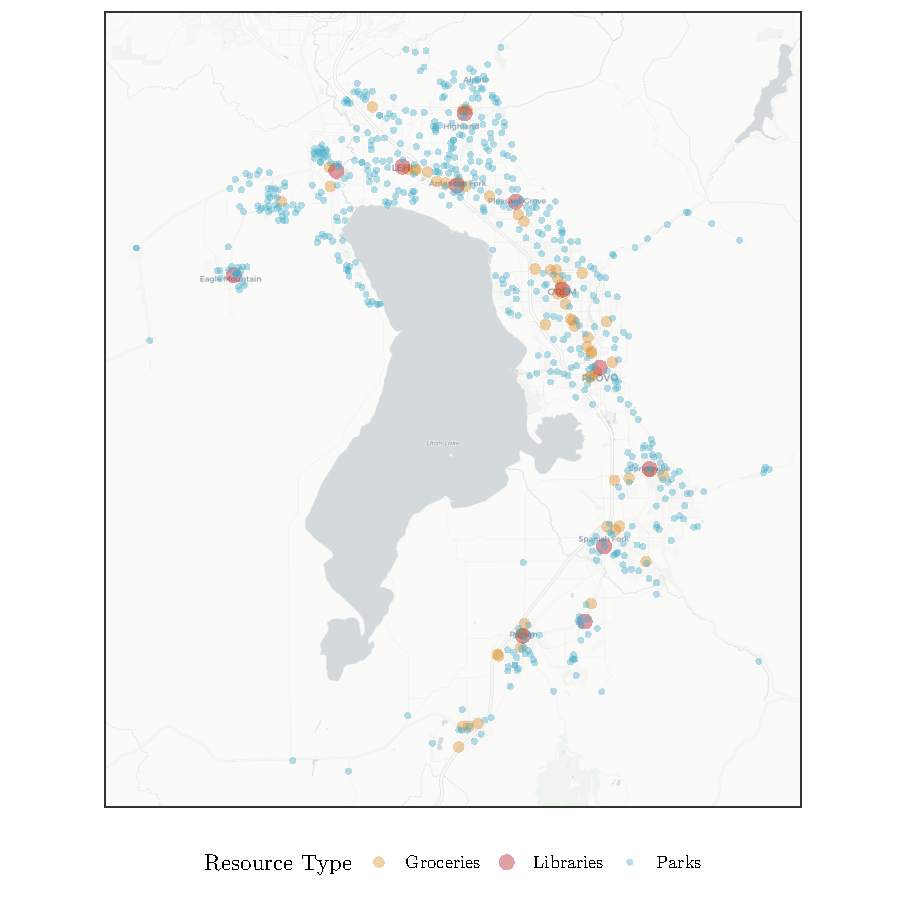
\includegraphics{Community_Resources_files/figure-latex/utco-map-1} 

}

\caption{Community Resources in Utah County}\label{fig:utco-map}
\end{figure}

\hypertarget{resource-data}{%
\subsubsection{Resource Data}\label{resource-data}}

Figure \ref{fig:utco-map} shows the locations of three types of
community resources in Utah County: parks, grocery stores, and libraries.
For each resource, and initial list of resources and elementary attributes was
obtained by executing a relevant query to OpenStreetMap (OSM).

Public parks and their attributes retrieved from OSM were verified and
corrected using aerial imagery and some site visits. The attributes included
the size of the park in acres, whether the park includes a playground, and
whether the park includes facilities for volleyball, basketball, and tennis.
The constructed dataset includes 582 attributed parks.

Grocery stores were retrieved from OSM and validated using internet resources and
site visits. The complete Nutritional Environment Measures Survey (NEMS-S) (\protect\hyperlink{ref-glanz2007}{Glanz et al., 2007})
was collected for each store, but this preliminary analysis only includes
cursory information on the stores including whether the store is a convenience store
or some other non-traditional grocery, whether the store includes a pharmacy or
other non-food merchandise, and the number of registers as a measure of the
store's size. The constructed dataset includes 58 stores.

Libraries were retrieved from OSM, and validated using library websites and
some site visits. The initial query returned university libraries and other
specialty resources; though some of these libraries are open to those outside
the university community, these were removed so that the resource list only
includes libraries generally catering to the general public. The amenities
available include whether the library offers additional classes and programs,
and whether the library includes genealogical or family history resources.
Other variables discussed in the literature such as the availability of computers
and public wi-fi networks were present in every library and therefore cannot
be included in the destination utility equations.

\hypertarget{mobile-device-data}{%
\subsubsection{Mobile Device Data}\label{mobile-device-data}}

\protect\hyperlink{ref-alamedaparks}{Macfarlane et al.} (\protect\hyperlink{ref-alamedaparks}{2021}) present a method for estimating destination choice models from
such data, which we repeat in this study. We provided a set of geometric
polygons for each park, grocery store, and library to StreetLight Data, Inc., a
commercial aggregator. StreetLight Data in turn provided data on the number of
mobile devices observed in each polygon grouped by the inferred residence block
group of of those devices during summer and fall 2019.
We then created a simulated destination choice estimation dataset for each
community resource by sampling 10,000 block group - resource ``trips'' from the
StreetLight dataset. This created a ``chosen'' alternative; we then sampled ten additional
resources at random (each simulated trip was paired with a different sample) to
serve as the non-chosen alternatives. Random sampling of alternatives is a
common practice that results in unbiased estimates, though the standard errors
of the estimates might be larger than could be obtained through a more carefully
designed sampling scheme (\protect\hyperlink{ref-train2009}{Train, 2009}).

\hypertarget{travel-times}{%
\subsubsection{Travel Times}\label{travel-times}}

Once the choice, alternatives, and attributes of the alternatives have been
defined, the last element of the choice utility is the travel impedance between
each block group and each resource. Using the \texttt{otpr} R interface (\protect\hyperlink{ref-otpr}{Marcus Young, 2020}) to
OpenTripPlanner, we estimated the highway drive travel time, the walking
route time, and the transit travel time for trips departing on October 1,
2021 at 8 AM. The time and date are most relevant for the transit path builder
in OpenTripPlanner, which uses detailed transit path information stored in the
Utah Transit Authority GTFS feed file for Fall 2021. The transit path contains
separate measures of the total travel time, the time in the transit vehicle,
transfer time, and access / egress time, allowing us full use of the
mode choice utility equations and resulting logsum described in Equation \eqref{eq:mcls}.

For groceries and libraries, we queried from OpenTripPlanner the shortest time path on each
mode from the population-weighted block group centroid to the centroid of the grocery
store or library centroid. Because some parks in the dataset can be relatively
large and the centroid might be far from the park access or use point, we instead
sampled points along the boundary of the park polygon, and queried the shortest
time path by each mode to the nearest boundary point.

\hypertarget{results}{%
\section{Results}\label{results}}

\hypertarget{destination-choice-models}{%
\subsection{Destination Choice Models}\label{destination-choice-models}}

Using the simulated trip choices assembled from the location-based services data,
we estimate destination choice models with the \texttt{mlogit} package for
R (\protect\hyperlink{ref-mlogit}{Croissant, 2020}; \protect\hyperlink{ref-R}{R Core Team, 2021}).

\begin{table}

\caption{\label{tab:park-models}Park Destination Choice Utilities}
\centering
\resizebox{\linewidth}{!}{
\begin{tabular}[t]{lccccc}
\toprule
  & Car & MCLS & Attributes & All - Car & All - Logsum\\
\midrule
Drive time & -0.215(-95.949)** &  &  & -0.209(-69.212)** & \\
Mode Choice Logsum &  & 7.678(95.958)** &  &  & 7.450(69.216)**\\
log(Acres) &  &  & 1.308(77.120)** & 1.300(46.869)** & 1.301(46.858)**\\
Playground &  &  & 4.567(33.939)** & 4.476(30.127)** & 4.477(30.118)**\\
Volleyball &  &  & -0.369(-9.580)** & -0.663(-11.065)** & -0.664(-11.067)**\\
Basketball &  &  & -0.669(-15.625)** & -0.534(-7.632)** & -0.535(-7.642)**\\
Tennis &  &  & -0.549(-13.065)** & -0.884(-14.678)** & -0.886(-14.693)**\\
\midrule
Num.Obs. & 8,984 & 8,984 & 8,984 & 8,984 & 8,984\\
Log Likelihood & -9,288.8 & -9,284.7 & -11,822.1 & -4,774.9 & -4,772.2\\
McFadden Rho-Sq & 0.569 & 0.569 & 0.451 & 0.778 & 0.778\\
\bottomrule
\multicolumn{6}{l}{\textsuperscript{} t-statistics in parentheses. * p $<$ 0.5, ** p $<$ 0.1}\\
\end{tabular}}
\end{table}

Table \ref{tab:park-models} presents the model estimation results for
five different specifications of park destination choice. The ``Car'' model
includes only the network travel time by car as a predictor of park choice;
the ``MCLS'' model similarly contains only the mode choice logsum as an
impedance term. The signs on the coefficient indicate that people are more
likely to choose parks with lower car distance or higher multi-modal access, all
else equal. The ``Attributes'' model includes only information on the park attributes
including size and amenities. On balance, people appear attracted to larger parks
and parks with playgrounds, while somewhat deterred by various sports facilities.
The ``All'' models include both the relevant travel impedance term as well as
destination attributes.

For most block group-park pairs, the transit and walk travel disutilities
are sufficiently high that choosing these travel modes is unlikely. As a
result, the mode choice logsum is highly collinear with the car travel time.
Nevertheless, there are small differences differences between the models
with the different impedance terms. Using a non-nested likelihood statistic
test presented by \protect\hyperlink{ref-horowitz1987}{Horowitz} (\protect\hyperlink{ref-horowitz1987}{1987}), we can reject the null hypothesis that the two
``All'' models have equivalent likelihood (\(p\)-value of 0.00969), and infer
that the mode choice logsum is a marginally better estimator of park choice than
the vehicle travel time alone.

\begin{table}

\caption{\label{tab:grocery-models}Grocery Destination Choice Utilities}
\centering
\resizebox{\linewidth}{!}{
\begin{tabular}[t]{lcccccc}
\toprule
  & Car & MCLS & Attributes & Size & All - Car & All - Logsum\\
\midrule
Drive time & -0.206(-90.014)** &  &  &  & -0.217(-78.388)** & \\
Mode Choice Logsum &  & 7.340(90.019)** &  &  &  & 7.733(78.399)**\\
Convenience Store &  &  & -2.339(-11.310)** & -1.600(-7.684)** & -1.486(-6.765)** & -1.488(-6.773)**\\
Other non-standard &  &  & -1.894(-14.604)** & -1.255(-9.554)** & -1.055(-7.487)** & -1.056(-7.490)**\\
Has pharmacy &  &  & 0.616(19.421)** & 0.329(8.901)** & 0.249(5.488)** & 0.249(5.502)**\\
Ethnic market &  &  & -1.680(-16.846)** & -0.997(-9.750)** & -0.883(-8.072)** & -0.884(-8.078)**\\
Has other merchandise &  &  & 1.523(48.309)** & 0.769(19.144)** & 0.881(17.631)** & 0.882(17.660)**\\
Number of registers &  &  &  & 0.073(42.117)** & 0.083(36.312)** & 0.083(36.294)**\\
Number of self-checkout &  &  &  & 0.031(15.255)** & 0.027(10.049)** & 0.027(10.041)**\\
\midrule
Num.Obs. & 8,404 & 8,404 & 8,404 & 8,404 & 8,404 & 8,404\\
Log Likelihood & -11,861 & -11,861.8 & -16,898.4 & -15,806.6 & -8,802.4 & -8,802.2\\
McFadden Rho-Sq & 0.411 & 0.411 & 0.161 & 0.216 & 0.563 & 0.563\\
\bottomrule
\multicolumn{7}{l}{\textsuperscript{} t-statistics in parentheses. * p $<$ 0.5, ** p $<$ 0.1}\\
\end{tabular}}
\end{table}

Table \ref{tab:grocery-models} presents the model estimation results for the grocery
store models. As with the parks models in Table \ref{tab:park-models}, the
most predictive model contains both a travel impedance term and attributes of
the destination grocery store. The number of registers suggests that people
prefer larger stores, all else equal; ethnic markets, convenience stores, and other
facilities are less preferred while stores with pharmacies and other merchandise
(clothes, home goods, etc.) attract visitors. The ratio of the drive time and
convenience store coefficients suggests that on average, people are willing to
drive 6.86 minutes to reach a store that is not a convenience store.
In terms of the travel impedance, there is not a sufficiently large gap in the
model likelihoods to reject that the mode choice logsum and the drive
time are equivalent predictors of grocery store choice.

\begin{table}

\caption{\label{tab:library-models}Library Destination Choice Utilities}
\centering
\resizebox{\linewidth}{!}{
\begin{tabular}[t]{lccccc}
\toprule
  & Car & MCLS & Attributes & All - Car & All - Logsum\\
\midrule
Drive time & -0.233(-95.379)** &  &  & -0.232(-89.281)** & \\
Mode Choice Logsum &  & 8.306(95.361)** &  &  & 8.270(89.266)**\\
Offers Classes &  &  & 1.318(44.405)** & 1.258(23.053)** & 1.257(23.033)**\\
Genealogy Resources &  &  & -1.127(-44.021)** & -1.024(-25.610)** & -1.024(-25.601)**\\
\midrule
Num.Obs. & 9,816 & 9,816 & 9,816 & 9,816 & 9,816\\
Log Likelihood & -10,841.9 & -10,840.3 & -21,944.4 & -10,322.5 & -10,321.7\\
McFadden Rho-Sq & 0.539 & 0.539 & 0.068 & 0.561 & 0.561\\
\bottomrule
\multicolumn{6}{l}{\textsuperscript{} t-statistics in parentheses. * p $<$ 0.5, ** p $<$ 0.1}\\
\end{tabular}}
\end{table}

Table \ref{tab:library-models} presents the model estimation results for the
library destination choice models. As with parks and grocery stores, both
travel impedance and destination attributes are significant predictors of
library choice. In this case, however, the library attributes provide very little
predictive power of library choice. This is perhaps because virtually all
libraries in the dataset offer the same set of basic amenities, but also because
each municipality in Utah County tends to operate its own library rather than
having a system of interconnected library branches as might be typical in
larger cities or other regions. Additionally, there is no significant difference
between the prediction power of the mode choice logsum versus the car travel
time.

\hypertarget{accessibilities}{%
\subsection{Accessibilities}\label{accessibilities}}

Using the results of the ``All - Logsum'' models estimated for each community resource
in the last section, we calculate the total utility-based accessibility measure
for each block group in Utah County. For comparison to a more traditional measure,
we also created buffer-based accessibility terms where a block group has
``access'' to a grocery store if there is one within a 5-minute drive, a
park if there is one within a five-minute walk, and a library if there is one within
a ten-minute drive.

\begin{figure}
\centering
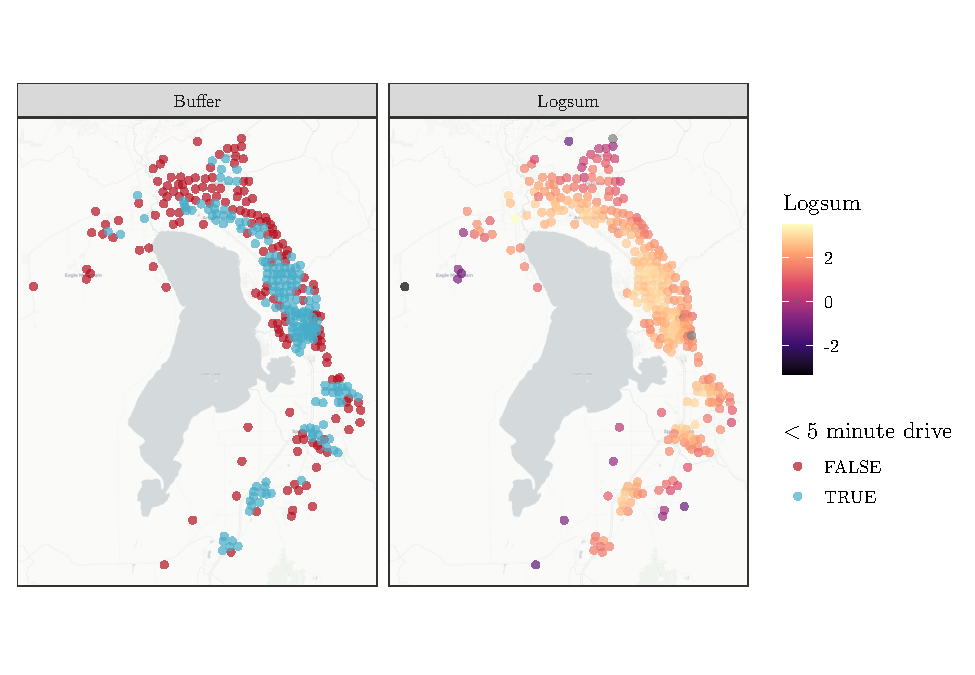
\includegraphics{Community_Resources_files/figure-latex/access-map-1.pdf}
\caption{\label{fig:access-map}Spatial comparison of grocery access buffer versus logsum.}
\end{figure}

Figure \ref{fig:access-map} spatially presents the difference between the
buffer-based measure and the logsum-based measure. The two measures largely
show the same basic shape: block groups along the spine of the county tend
to have binary access in the buffer and also have a higher logsum value. The
difference is at the margins, where the discontinuity of the buffer measure
is replaced by a smoother access surface, more spatially reflective of what
people are likely to experience.

\begin{figure}
\centering
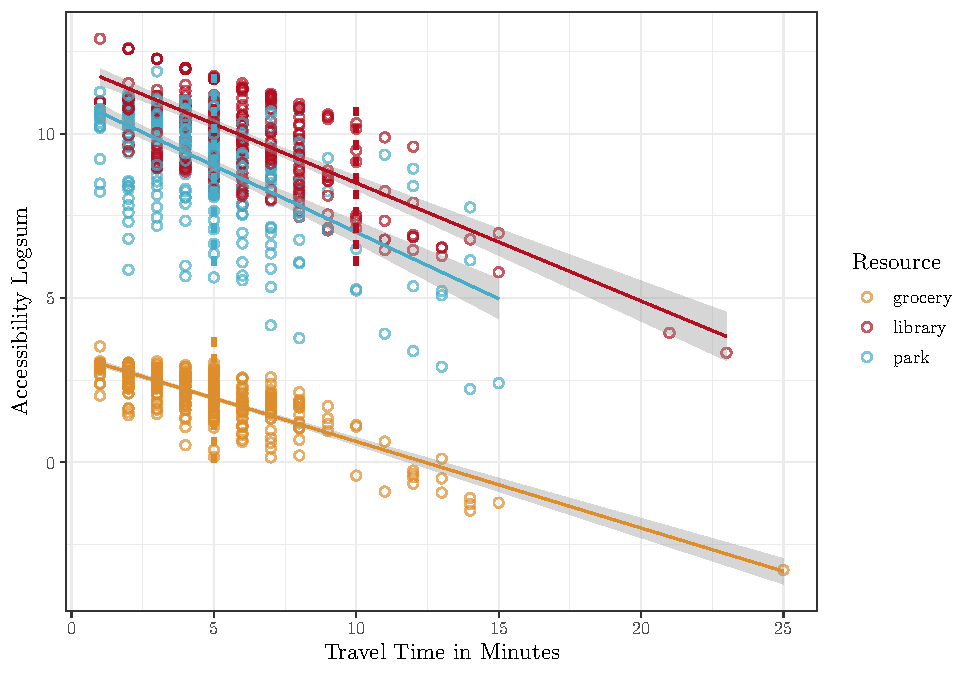
\includegraphics{Community_Resources_files/figure-latex/access-plot-1.pdf}
\caption{\label{fig:access-plot}Relationship between travel time, and logsum access value for block groups in Utah County. Travel-time based buffers shown as dashed lines.}
\end{figure}

The potential for the buffer measure to oversimplify the accessiblity problem is further
illustrated in
Figure \ref{fig:access-plot}. This figure shows the utility-based accessibility
logsum calculated using the mode choice logsum as an impedance term against the
travel time in minutes (drive time for grocery stores and libraries; walk time
for parks), for block groups in the study region. It is clear that for all three
land uses,
lower travel time is significantly correlated with higher accessibility.
But for block groups with with equivalent travel time to a particular community
resource, the accessibility logsum value
varies substantially. Even for block groups along the buffer --- where a small change
in travel time might place a block within or without the buffer --- the variance
in accessibility logsum appears to be almost as large as the variance as the variance
in the travel time. This variance in accessiblity logsum might be due to a
travel time differential between drive, walk, and transit modes captured in the
mode choice logsum, or it could also be because the resources available near the
set of block groups have substantial variance in their amenities. Being near a
single poor-quality grocery store is not the same thing as being near multiple
high-quality groceries, and the logsum value can capture this variance in its
construction.

What this distinction between access estimation methods might mean for policy
analysis is yet to be determined, and future research is required. In this analysis,
we estimate that 26,107 households live in block groups outside the
boundary of all three resource buffers: 10-minute drive for a library, 5-minute drive for
a grocery store, and 5-minute walk for a park. Of these, 2,385 make less
than \$35,000 per year.
At the same time, only 17,932 households
live in block groups that are beneath the regional mean utility-based access to
all three resources; that is, they have less-than the regional average access to
grocery stores, and to libraries, and to parks. Of these households, 1,633
are similarly low-income. Perhaps more importantly, the overlap between the households
in \emph{both} groups is not very high: only 9,510 households live
in block groups with low access determined by both buffers and by accessiblity
logsum, 831 of which are low-income households.

\hypertarget{limitations-and-future-research}{%
\section{Limitations and Future Research}\label{limitations-and-future-research}}

The location-based services data reveals the likely home location of devices
observed within a geographic polygon, within some measurement error.
It cannot tell us whether the device holder actually accomplished the assumed
activity; that is, there may be a reason why a device was observed near a
library even though the person did not actually patronize the library.
Additionally, the method we use to compile the estimation dataset presumes that
the choice to make a trip to the community resource has already been made. Though
it can suggest how the accessibility of a neighborhood to these resource would improve
were transportation impedance decreased or the resources expanded or improved,
it cannot tell us how many more people might take advantage of the resource
in that case.

In this research, all simulated trips were grouped into a single pooled model
for analysis. This implies that the effect of amenities and travel impedance on
destination choice is similar for all neighborhoods. A segmented model
where, for example, low-income block groups and high-income block groups were
estimated separately could allow for flexibility in these estimates and reveal
differences in preferences among residents of the different neighborhoods. Some
neighborhoods might show a particular preference for access utilities by
transit, or for specific park amenities. A latent class choice model (\protect\hyperlink{ref-walker2002}{Walker and Ben-Akiva, 2002})
would go further in potentially informing which demographic variables are
meaningful in defining possible data segmentation schemes.

A necessary assumption made when constructing the estimation dataset is that
people experience access from their home neighborhood. This may not always be true;
for instance, people may choose to shop at grocery stores or visit libraries that
are near their workplace, or that are between their homes and some other
frequent destination. Methods to account for access and destination choices
experienced at other points in the day would be a useful and interesting extension.
Similarly, we assumed that the distance between a home and a community resource
was represented by the distance between the block group centroid and the resource.
For some block groups in less dense areas of the county, the error in measured
travel time between the block group centroid and the actual home location might be
larger than the total travel time. It might be possible to simulate home locations
within each block group and use those locations in the travel time calculations.
Alternatively, it might be possible to estimate the model using block group data
as in this study but apply the model at a more fine resolution (e.g.~block) when
investigating accessibilities and conducting policy analyses.

This paper presents preliminary model estimates using plausible destination
choice utility values. Several additional variables might be further explored,
particularly in regards to the grocery resources. The NEMS-S survey is a highly
detailed picture of the offerings of a particular grocery store, including
information on the availability of relatively healthier or fresher foods and
their prices. This study was only able to explore a few key size variables, but
a deeper investigation into grocery store amenities and offerings
preferences --- and how they might influence a collective understanding of
nutrition access more broadly --- is needed.

\hypertarget{conclusions}{%
\section{Conclusions}\label{conclusions}}

This paper developed accessibility-based measures of accessibility to three
types of community resource: parks, grocery stores, and libraries. These metrics
were informed by observing trips to specific facilities in mobile
device data, allowing the measures to incorporate attributes of the resource
as well as attributes of the journey there. The computed measures are
fundamentally different from buffer-based measures more commonly used to
inform spatial policy analysis.

Ultimately, the purpose of any accessibility measure to a community resources
is to enable a subsequent analysis of some metric of well-being. \protect\hyperlink{ref-macfarlane2020}{Macfarlane et al.} (\protect\hyperlink{ref-macfarlane2020}{2020})
suggest that a utility-based access to parks measure is more predictive of
physical health outcomes than a buffer-based measure. Is this true for more
community resources? Would using a more subtle or nuanced measure of access to
libraries help in understanding a link between community form and social isolation
or mental health? A key benefit of this method is that is provides a way to
evaluate the benefit of investments in resources against the benefits of investing
in the transportation system. Will a community benefit more from a new grocery store
nearby, or expanded options at an existing grocery store, or from improving bike
or bus connections to that existing store? An examination of this question is
left for future research, but this paper presents a method for how this could be
approached.

\hypertarget{acknowledgements}{%
\section*{Acknowledgements}\label{acknowledgements}}
\addcontentsline{toc}{section}{Acknowledgements}

The authors are grateful to Alisha Redelfs, Lori Spruance, Kaeli Monahan, and
Mali Smith for their help in gathering the grocery store information data.
Connor Williams gathered the parks data. Tables and figures in the article are
produced using a variety of packages for R (\protect\hyperlink{ref-modelsummary}{Arel-Bundock, 2021}; \protect\hyperlink{ref-ggspatial}{Dunnington, 2021})

\hypertarget{references}{%
\section*{References}\label{references}}
\addcontentsline{toc}{section}{References}

\hypertarget{refs}{}
\begin{CSLReferences}{1}{0}
\leavevmode\vadjust pre{\hypertarget{ref-aggarwal2014}{}}%
Aggarwal, A., Cook, A.J., Jiao, J.F., Seguin, R.A., Moudon, A.V., Hurvitz, P.M., Drewnowski, A., 2014. Access to supermarkets and fruit and vegetable consumption. \emph{American Journal of Public Health} 104, 917--923. \url{https://doi.org/10.2105/Ajph.2013.301763}

\leavevmode\vadjust pre{\hypertarget{ref-algert2006}{}}%
Algert, S.J., Agrawal, A., Lewis, D.S., 2006. Disparities in access to fresh produce in low-income neighborhoods in los angeles. \emph{American Journal of Preventive Medicine} 30, 365--370. \url{https://doi.org/10.1016/j.amepre.2006.01.009}

\leavevmode\vadjust pre{\hypertarget{ref-allen2019}{}}%
Allen, J., 2019. Mapping differences in access to public libraries by travel mode and time of day. \emph{Library \& Information Science Research} 41, 11--18. \url{https://doi.org/10.1016/j.lisr.2019.02.001}

\leavevmode\vadjust pre{\hypertarget{ref-modelsummary}{}}%
Arel-Bundock, V., 2021. Modelsummary: Summary tables and plots for statistical models and data: Beautiful, customizable, and publication-ready.

\leavevmode\vadjust pre{\hypertarget{ref-bancroft2015association}{}}%
Bancroft, C., Joshi, S., Rundle, A., Hutson, M., Chong, C., Weiss, C.C., Genkinger, J., Neckerman, K., Lovasi, G., 2015. Association of proximity and density of parks and objectively measured physical activity in the united states: A systematic review. \emph{Social science \& medicine} 138, 22--30.

\leavevmode\vadjust pre{\hypertarget{ref-barclay2017space}{}}%
Barclay, D.A., 2017. Space and the social worth of public libraries. \emph{Public library quarterly} 36, 267--273.

\leavevmode\vadjust pre{\hypertarget{ref-bedimo2005}{}}%
Bedimo-Rung, A.L., Mowen, A.J., Cohen, D.A., 2005. The significance of parks to physical activity and public health. \emph{American Journal of Preventive Medicine} 28, 159--168. \url{https://doi.org/10.1016/j.amepre.2004.10.024}

\leavevmode\vadjust pre{\hypertarget{ref-nchrp716}{}}%
Cambridge Systematics, 2012. Travel demand forecasting: Parameters and techniques (NCHRP Report No. 716). Transportation Research Board.

\leavevmode\vadjust pre{\hypertarget{ref-chen2021effects}{}}%
Chen, Z., Yeh, A.G.-O., 2021. Effects of built environment on activity participation under different space-time constraints: A case study of guangzhou, china. \emph{Travel Behaviour and Society} 22, 84--93.

\leavevmode\vadjust pre{\hypertarget{ref-cheng2021}{}}%
Cheng, W., Wu, J., Moen, W., Hong, L., 2021. Assessing the spatial accessibility and spatial equity of public libraries' physical locations. \emph{Library \& Information Science Research} 43, 101089. https://doi.org/\url{https://doi.org/10.1016/j.lisr.2021.101089}

\leavevmode\vadjust pre{\hypertarget{ref-clifton2004}{}}%
Clifton, K.J., 2004. Mobility strategies and food shopping for low-income families - a case study. \emph{Journal of Planning Education and Research} 23, 402--413. \url{https://doi.org/10.1177/0739456x04264919}

\leavevmode\vadjust pre{\hypertarget{ref-mlogit}{}}%
Croissant, Y., 2020. Estimation of random utility models in {R}: The {mlogit} package. \emph{Journal of Statistical Software} 95, 1--41. \url{https://doi.org/10.18637/jss.v095.i11}

\leavevmode\vadjust pre{\hypertarget{ref-dong2006}{}}%
Dong, X.J., Ben-Akiva, M.E., Bowman, J.L., Walker, J.L., 2006. Moving from trip-based to activity-based measures of accessibility. \emph{Transportation Research Part a-Policy and Practice} 40, 163--180. \url{https://doi.org/10.1016/j.tra.2005.05.002}

\leavevmode\vadjust pre{\hypertarget{ref-ggspatial}{}}%
Dunnington, D., 2021. Ggspatial: Spatial data framework for ggplot2.

\leavevmode\vadjust pre{\hypertarget{ref-ermagun2020}{}}%
Ermagun, A., Tilahun, N., 2020. Equity of transit accessibility across chicago. \emph{Transportation Research Part D: Transport and Environment} 86, 102461. \url{https://doi.org/10.1016/j.trd.2020.102461}

\leavevmode\vadjust pre{\hypertarget{ref-glanz2007}{}}%
Glanz, K., Sallis, J.F., Saelens, B.E., Frank, L.D., 2007. Nutrition environment measures survey in stores (NEMS-s): Development and evaluation. \emph{American journal of preventive medicine} 32, 282--289.

\leavevmode\vadjust pre{\hypertarget{ref-guo2017}{}}%
Guo, Y., Chan, C.H., Yip, P.S.F., 2017. Spatial variation in accessibility of libraries in hong kong. \emph{Library \& Information Science Research} 39, 319--329. https://doi.org/\url{https://doi.org/10.1016/j.lisr.2017.11.007}

\leavevmode\vadjust pre{\hypertarget{ref-hamidi2020}{}}%
Hamidi, S., 2020. Urban sprawl and the emergence of food deserts in the USA. \emph{Urban Studies} 57, 1660--1675. \url{https://doi.org/10.1177/0042098019841540}

\leavevmode\vadjust pre{\hypertarget{ref-handy1997}{}}%
Handy, S.L., Niemeier, D.A., 1997. Measuring accessibility: An exploration of issues and alternatives. \emph{Environment and planning A} 29, 1175--1194.

\leavevmode\vadjust pre{\hypertarget{ref-hansen1959}{}}%
Hansen, W.G., 1959. How accessibility shapes land use. \emph{Journal of the American Institute of Planners} 25, 73--76. \url{https://doi.org/10.1080/01944365908978307}

\leavevmode\vadjust pre{\hypertarget{ref-horowitz1987}{}}%
Horowitz, J.L., 1987. Specification tests for nested logit models. \emph{Environment and Planning A: Economy and Space} 19, 395--402. \url{https://doi.org/10.1068/a190395}

\leavevmode\vadjust pre{\hypertarget{ref-kacynski2016}{}}%
Kaczynski, A.T., Schipperijn, J., Hipp, J.A., Besenyi, G.M., Wilhelm Stanis, S.A., Hughey, S.M., Wilcox, S., 2016. ParkIndex: Development of a standardized metric of park access for research and planning. \emph{Preventive Medicine} 87, 110--114. \url{https://doi.org/10.1016/j.ypmed.2016.02.012}

\leavevmode\vadjust pre{\hypertarget{ref-kinnell2006}{}}%
Kinnell, J.C., Bingham, M.F., Mohamed, A.F., Desvousges, W.H., Kiler, T.B., Hastings, E.K., Kuhns, K.T., 2006. Estimating site choice decisions for urban recreators. \emph{Land Economics} 82, 257--272. \url{https://doi.org/10.3368/le.82.2.257}

\leavevmode\vadjust pre{\hypertarget{ref-lochner1999}{}}%
Lochner, K., 1999. Social capital: A guide to its measurement. \emph{Health \& Place} 5, 259--270. \url{https://doi.org/10.1016/s1353-8292(99)00016-7}

\leavevmode\vadjust pre{\hypertarget{ref-logan2019}{}}%
Logan, T.M., Williams, T.G., Nisbet, A.J., Liberman, K.D., Zuo, C.T., Guikema, S.D., 2019. Evaluating urban accessibility: Leveraging open-source data and analytics to overcome existing limitations. \emph{Environment and Planning B-Urban Analytics and City Science} 46, 897--913. \url{https://doi.org/10.1177/2399808317736528}

\leavevmode\vadjust pre{\hypertarget{ref-macfarlane2020}{}}%
Macfarlane, G.S., Boyd, N., Taylor, J.E., Watkins, K., 2020. Modeling the impacts of park access on health outcomes: A utility-based accessibility approach. \emph{Environment and Planning B: Urban Analytics and City Science}. \url{https://doi.org/10.1177/2399808320974027}

\leavevmode\vadjust pre{\hypertarget{ref-alamedaparks}{}}%
Macfarlane, G.S., Turley Voulgaris, C., Tapia, T., 2021. If you build it who will come? Equity analysis of park system changes during COVID-19 using passive origin-destination data. \emph{Journal of Transport and Land Use}.

\leavevmode\vadjust pre{\hypertarget{ref-otpr}{}}%
Marcus Young, 2020. {otpr: An API wrapper for OpenTripPlanner}. \url{https://doi.org/10.5281/zenodo.4065250}

\leavevmode\vadjust pre{\hypertarget{ref-maxwell2008libraries}{}}%
Maxwell, N.K., 2008. Libraries?---yes, in my backyard! \emph{Journal of access services} 5, 391--396.

\leavevmode\vadjust pre{\hypertarget{ref-monz2019}{}}%
Monz, C., Mitrovich, M., D'Antonio, A., Sisneros-Kidd, A., 2019. {Using Mobile Device Data to Estimate Visitation in Parks and Protected Areas: An Example from the Nature Reserve of Orange County, California}. \emph{Journal of Park and Recreation Administration}. \url{https://doi.org/10.18666/JPRA-2019-9899}

\leavevmode\vadjust pre{\hypertarget{ref-morland2002}{}}%
Morland, K., Wing, S., Roux, A.D., Poole, C., 2002. Neighborhood characteristics associated with the location of food stores and food service places. \emph{American Journal of Preventive Medicine} 22, 23--29. \url{https://doi.org/Pii\%20S0749-377(01)00403-2\%0ADoi\%2010.1016/S0749-3797(01)00403-2}

\leavevmode\vadjust pre{\hypertarget{ref-muth1971}{}}%
Muth, R.F., 1971. The derived demand for urban residential land. \emph{Urban studies} 8, 243--254.

\leavevmode\vadjust pre{\hypertarget{ref-naboulsi2016}{}}%
Naboulsi, D., Fiore, M., Ribot, S., Stanica, R., 2016. Large-scale mobile traffic analysis: A survey. \emph{IEEE Communications Surveys \& Tutorials} 18, 124--161. \url{https://doi.org/10.1109/comst.2015.2491361}

\leavevmode\vadjust pre{\hypertarget{ref-neusel2016}{}}%
Neusel Ussery, E., Yngve, L., Merriam, D., Whitfield, G., Foster, S., Wendel, A., Boehmer, T., 2016. The national environmental public health tracking network access to parks indicator: A national county-level measure of park proximity. \emph{Journal of Park and Recreation Administration} 34. \url{https://doi.org/10.18666/jpra-2016-v34-i3-7119}

\leavevmode\vadjust pre{\hypertarget{ref-philbin2019}{}}%
Philbin, M.M., Parker, C.M., Flaherty, M.G., Hirsch, J.S., 2019. Public libraries: A community-level resource to advance population health. \emph{Journal of Community Health} 44, 192--199. \url{https://doi.org/10.1007/s10900-018-0547-4}

\leavevmode\vadjust pre{\hypertarget{ref-R}{}}%
R Core Team, 2021. R: A language and environment for statistical computing. R Foundation for Statistical Computing, Vienna, Austria.

\leavevmode\vadjust pre{\hypertarget{ref-recker1978}{}}%
Recker, W.W., Kostyniuk, L.P., 1978. Factors influencing destination choice for the urban grocery shopping trip. \emph{Transportation} 7, 19--33.

\leavevmode\vadjust pre{\hypertarget{ref-rigolon2018}{}}%
Rigolon, A., Browning, M., Jennings, V., 2018. Inequities in the quality of urban park systems: An environmental justice investigation of cities in the united states. \emph{Landscape and Urban Planning} 178, 156--169. \url{https://doi.org/10.1016/j.landurbplan.2018.05.026}

\leavevmode\vadjust pre{\hypertarget{ref-train2009}{}}%
Train, K.E., 2009. {Discrete Choice Methods with Simulation, 2nd Edition}. Cambridge University Press, Cambridge. \url{https://doi.org/10.1016/S0898-1221(04)90100-9}

\leavevmode\vadjust pre{\hypertarget{ref-parkscore2019}{}}%
Trust for Public Land, 2019. {2019 ParkScore Index}.

\leavevmode\vadjust pre{\hypertarget{ref-usdafara}{}}%
U.S. Department of Agriculture, 2021. Food access research atlas.

\leavevmode\vadjust pre{\hypertarget{ref-walker2002}{}}%
Walker, J., Ben-Akiva, M., 2002. Generalized random utility model. \emph{Mathematical Social Sciences} 43, 303--343. \url{https://doi.org/Pii\%20S0165-4896(02)00023-9\%0ADoi\%2010.1016/S0165-4896(02)00023-9}

\leavevmode\vadjust pre{\hypertarget{ref-tidycensus}{}}%
Walker, K., Herman, M., 2021. Tidycensus: Load US census boundary and attribute data as 'tidyverse' and 'sf'-ready data frames.

\leavevmode\vadjust pre{\hypertarget{ref-widener2015spatiotemporal}{}}%
Widener, M.J., Farber, S., Neutens, T., Horner, M., 2015. Spatiotemporal accessibility to supermarkets using public transit: An interaction potential approach in cincinnati, ohio. \emph{Journal of Transport Geography} 42, 72--83.

\leavevmode\vadjust pre{\hypertarget{ref-williams1977formation}{}}%
Williams, H.C., 1977. On the formation of travel demand models and economic evaluation measures of user benefit. \emph{Environment and planning A} 9, 285--344.

\leavevmode\vadjust pre{\hypertarget{ref-witten2003}{}}%
Witten, K., Exeter, D., Field, A., 2003. The quality of urban environments: Mapping variation in access to community resources. \emph{Urban Studies} 40, 161--177. \url{https://doi.org/10.1080/00420980220080221}

\leavevmode\vadjust pre{\hypertarget{ref-wood2016}{}}%
Wood, B.S., Horner, M.W., 2016. Understanding accessibility to snap-accepting food store locations: Disentangling the roles of transportation and socioeconomic status. \emph{Applied Spatial Analysis and Policy} 9, 309--327. \url{https://doi.org/10.1007/s12061-015-9138-2}

\leavevmode\vadjust pre{\hypertarget{ref-tcrp138}{}}%
Zalewski, A., Sonenklar, D., Cohen, A., Kressner, J., Macfarlane, G., 2019. Public transit rider origin-destination survey methods and technologies (TCRP Synthesis Report No. 138). Transportation Research Board.

\leavevmode\vadjust pre{\hypertarget{ref-zhu2018}{}}%
Zhu, J., Ye, X., 2018. Development of destination choice model with pairwise district-level constants using taxi GPS data. \emph{Transportation Research Part C: Emerging Technologies} 93, 410--424. \url{https://doi.org/10.1016/j.trc.2018.06.016}

\end{CSLReferences}


\end{document}
